\documentclass[pdftex,11pt]{beamer}
%\documentclass[trans]{beamer}

\usepackage[T1]{fontenc}
\usepackage[utf8]{inputenc}
\usepackage{lmodern}
\usepackage{multirow}
\usepackage{amsbsy}
\usepackage{fixmath}
\usepackage{amssymb,amsmath,latexsym}
\usepackage{tikz}
\usepackage{graphicx}
%\usepackage{algorithmic}
%\usepackage[ruled,vlined]{algorithm2e}
%\usepackage{algorithm2e}

\usetikzlibrary{shapes.misc}
\usetikzlibrary{shapes.arrows}
\usetikzlibrary{shapes.geometric}
\usetikzlibrary{decorations.pathreplacing}
\usetikzlibrary{decorations.pathmorphing}
\usetikzlibrary{backgrounds}
\usetikzlibrary{matrix}
\usetikzlibrary{fit}
\usetikzlibrary{calc}


%% Output fonts encoding

\usefonttheme{professionalfonts}

%% Title informations
\title{Reference-Based Transcriptome Assembly}

\author{Mingfu Shao}

\institute{Computational Biology Department, Carnegie Mellon University}
\date{\today}

%% Specific packages


%% Theme
\usetheme{LANE}

%% Figures
\thinlines
\setlength{\unitlength}{1mm}
\linethickness{0.3mm}

%%%%%%%%%%%%%%%%%%%%%%
\begin{document}
%%%%%%%%%%%%%%%%%%%%%%

\AtBeginSection[] {
	\begin{frame}[plain]
		\frametitle{Outline}
	\tableofcontents[currentsection]
		\end{frame}
	\addtocounter{framenumber}{-1}
}

%\frame{\titlepage}

%\frame
%{
%	\frametitle{Outline}
%	\tableofcontents
%}

\frame
{
	\frametitle{RNA-seq Experiments}

	\vspace{-0.05cm}
	\begin{columns}[c]
	\column{0.48\textwidth} 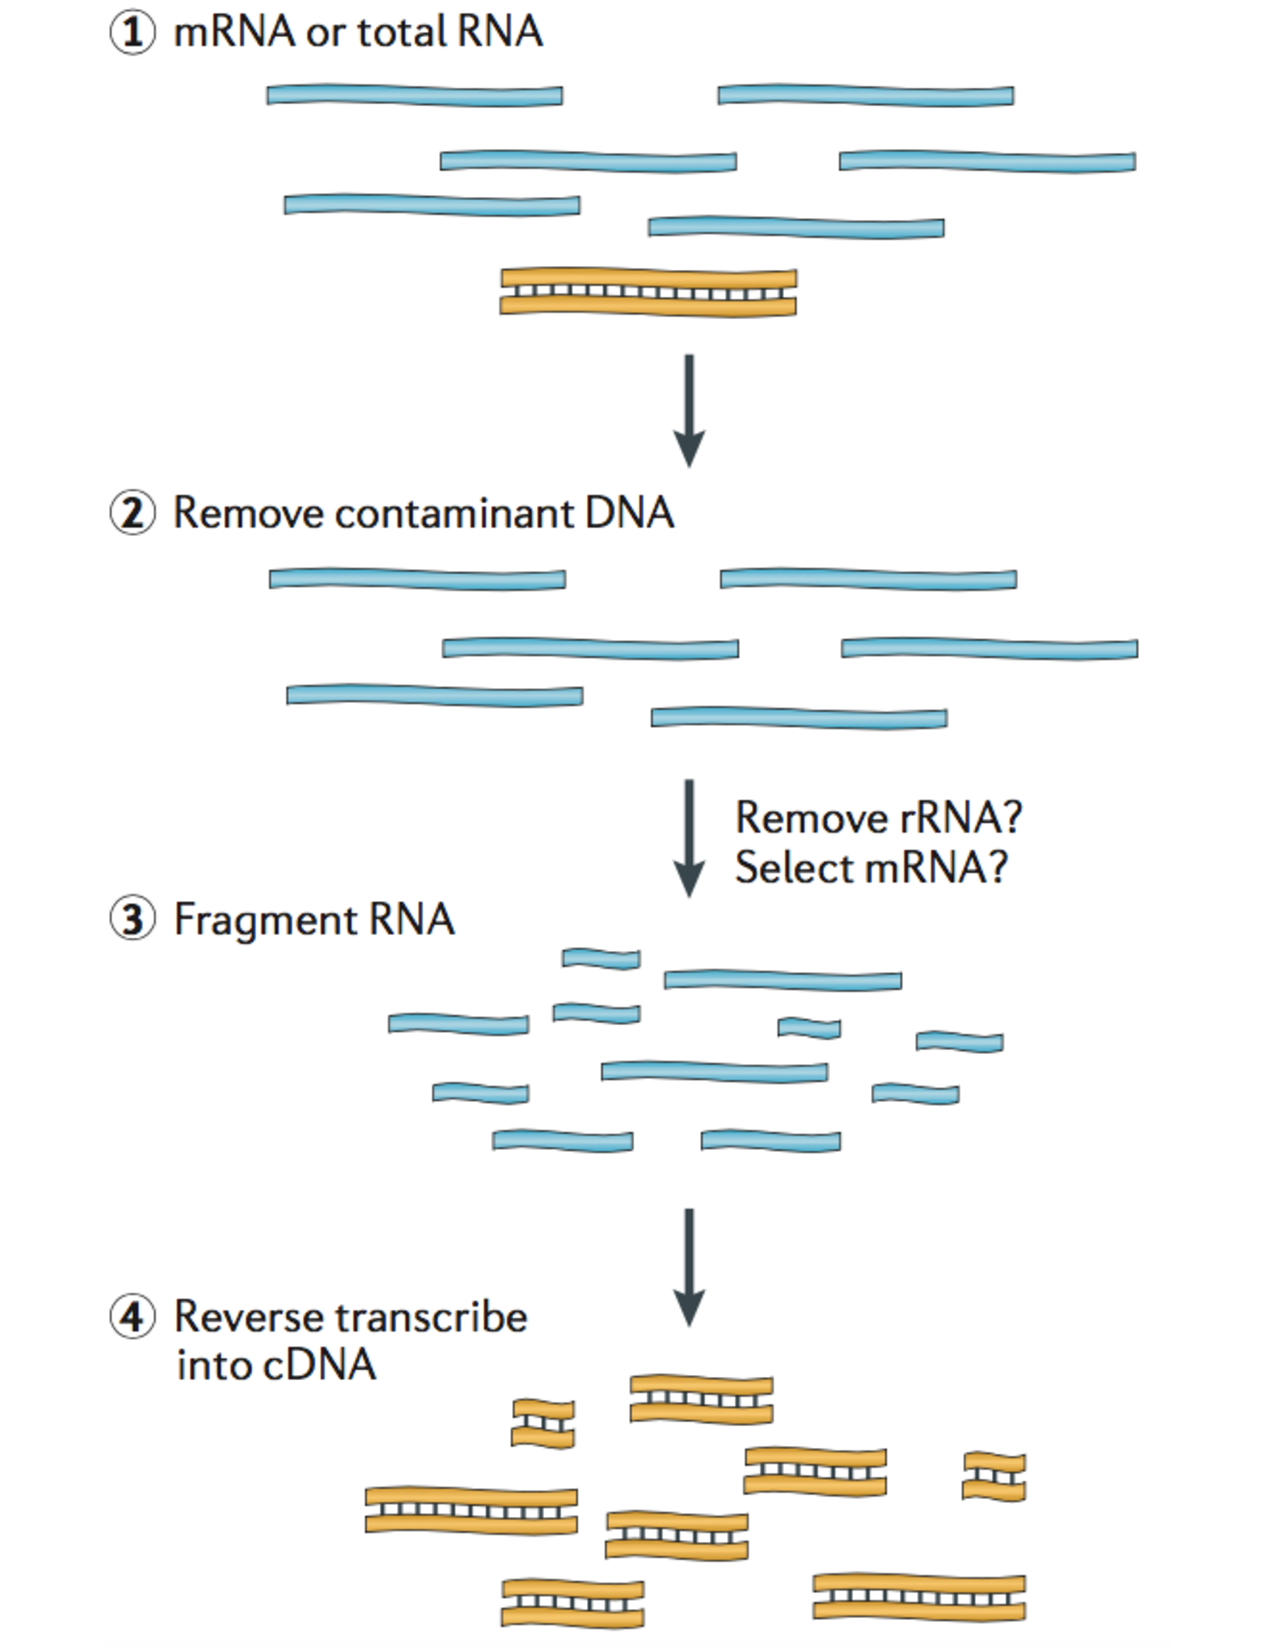
\includegraphics[width=\textwidth]{figures/seq1.pdf}
	\column{0.48\textwidth} 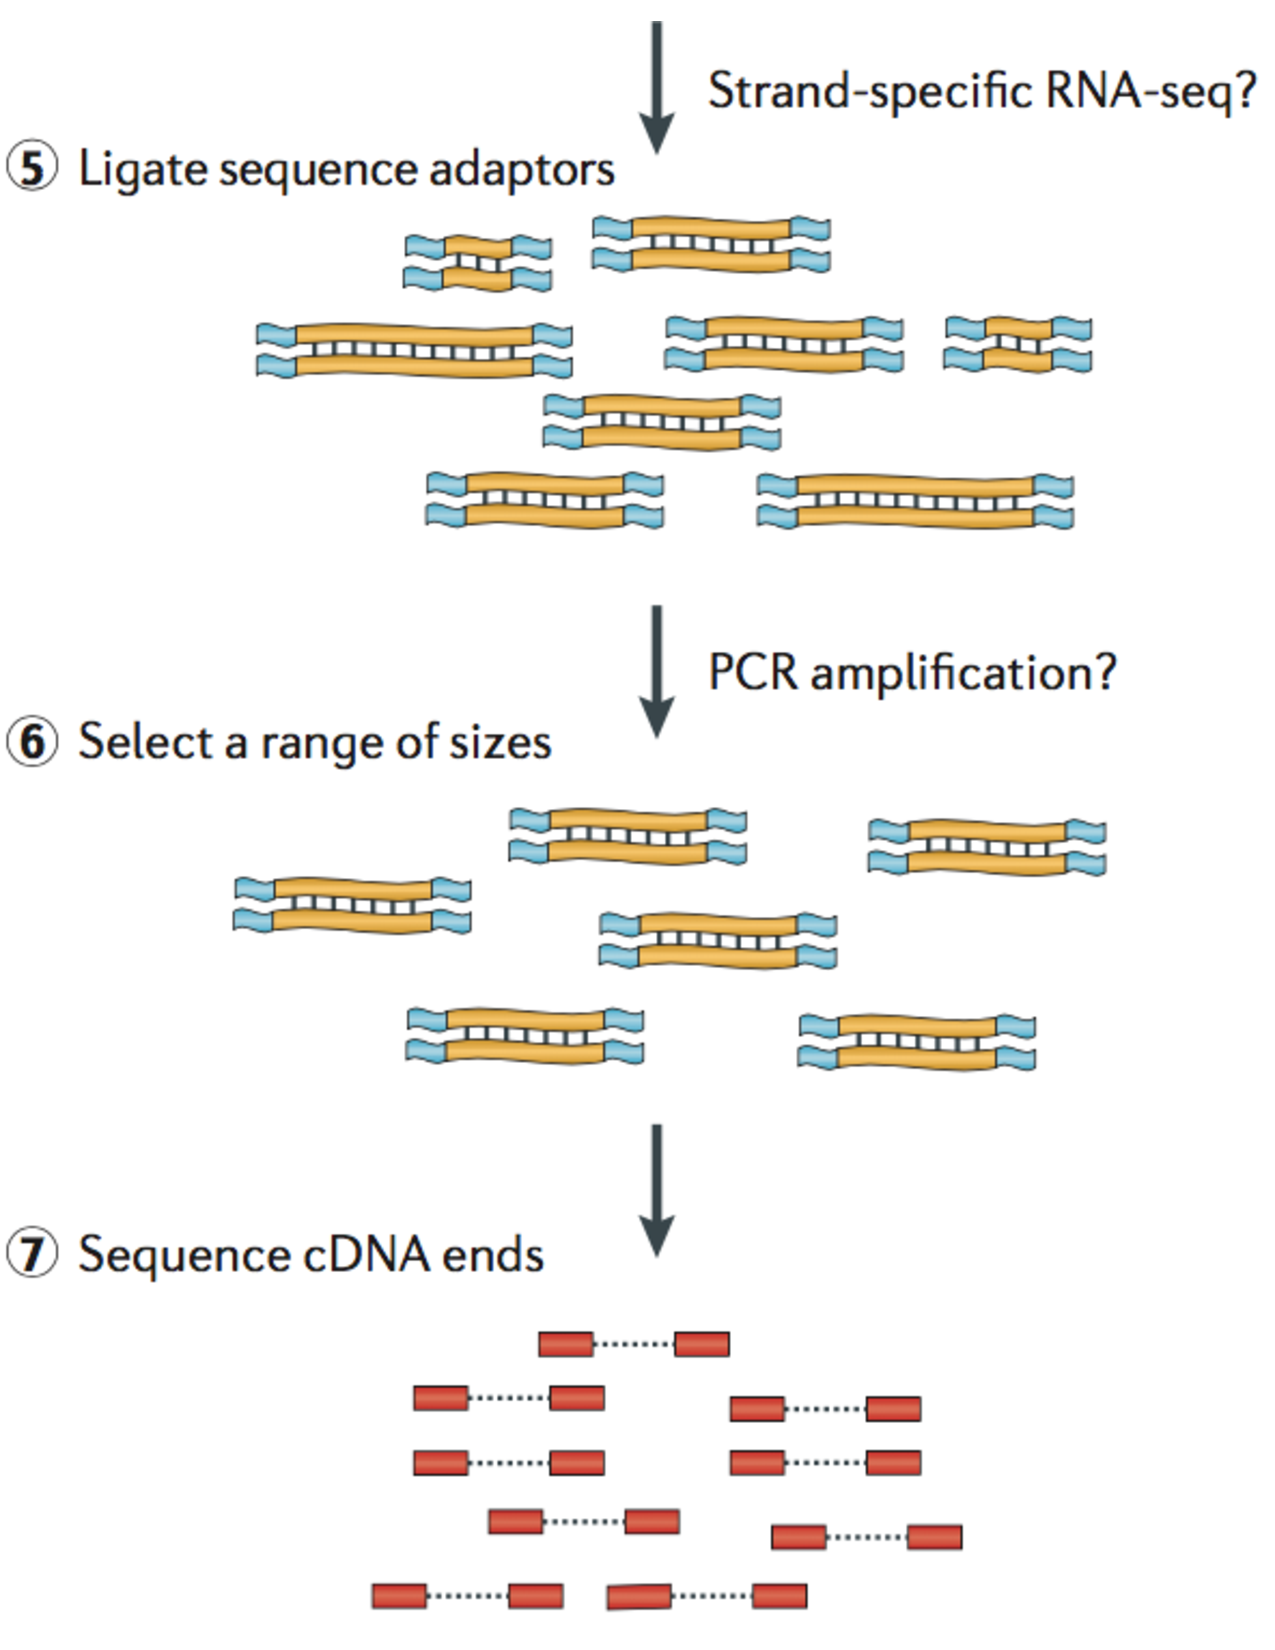
\includegraphics[width=\textwidth]{figures/seq2.pdf}
	\end{columns}

	\vspace{0.25cm}
	\onslide<2->{{\bf Transcriptome Assembly:} To determine the transcripts and their abundance from the (paired-end) reads.}
}

\frame
{
	\frametitle{Existing Softwares/Methods}
	\begin{itemize}
	\item {\bf Reference-based} methods:
		\vspace{0.05cm}
		\begin{itemize}
		\item Cufflinks~(Trapnell \emph{et al.}, 2010) \hspace{0.7cm}\onslide<2->{{\bf use overlap graph}}
		\vspace{-0.05cm}
		\[\left.\hspace{-0.98cm}\parbox{0.5\textwidth}{%
		\item Scripture~(Guttman \emph{et al.}, 2010)
		\vspace{0.05cm}
		\item IsoLasso~(Li \emph{et al.}, 2011)
		\vspace{0.05cm}
		\item SLIDE~(Li \emph{et al.}, 2011)
		\vspace{0.05cm}
		\item CLIIQ~(Lin \emph{et al.}, 2012)
		\vspace{0.05cm}
		\item CEM~(Li \emph{et al.}, 2012)
		\vspace{0.05cm}
		\item MITIE~(Behr \emph{et al.}, 2013)
		\vspace{0.05cm}
		\item Traph~(Tomescu \emph{et al.}, 2013)
		\vspace{0.05cm}
		\item StringTie~(Pertea \emph{et al.}, 2015)}
		\onslide<2->{\right\} \textsf{\bf use splice graph}}\]
		\vspace{-0.2cm}
		\item {\bf ...}
		\end{itemize}
	\vspace{0.2cm}
	\item {\bf\emph{De novo}} methods:
		\vspace{0.05cm}
		\begin{itemize}
		\item Trans-ABySS~(Robertson \emph{et al.}, 2010)
		\vspace{0.05cm}
		\item Trinity~(Grabherr \emph{et al.}, 2011)
		\vspace{0.05cm}
		\item Oases~(Schulz \emph{et al.}, 2012)
		\vspace{0.05cm}
		\item {\bf ...}
		\end{itemize}
	\end{itemize}
}

\frame
{
	\frametitle{Splice Graph}
	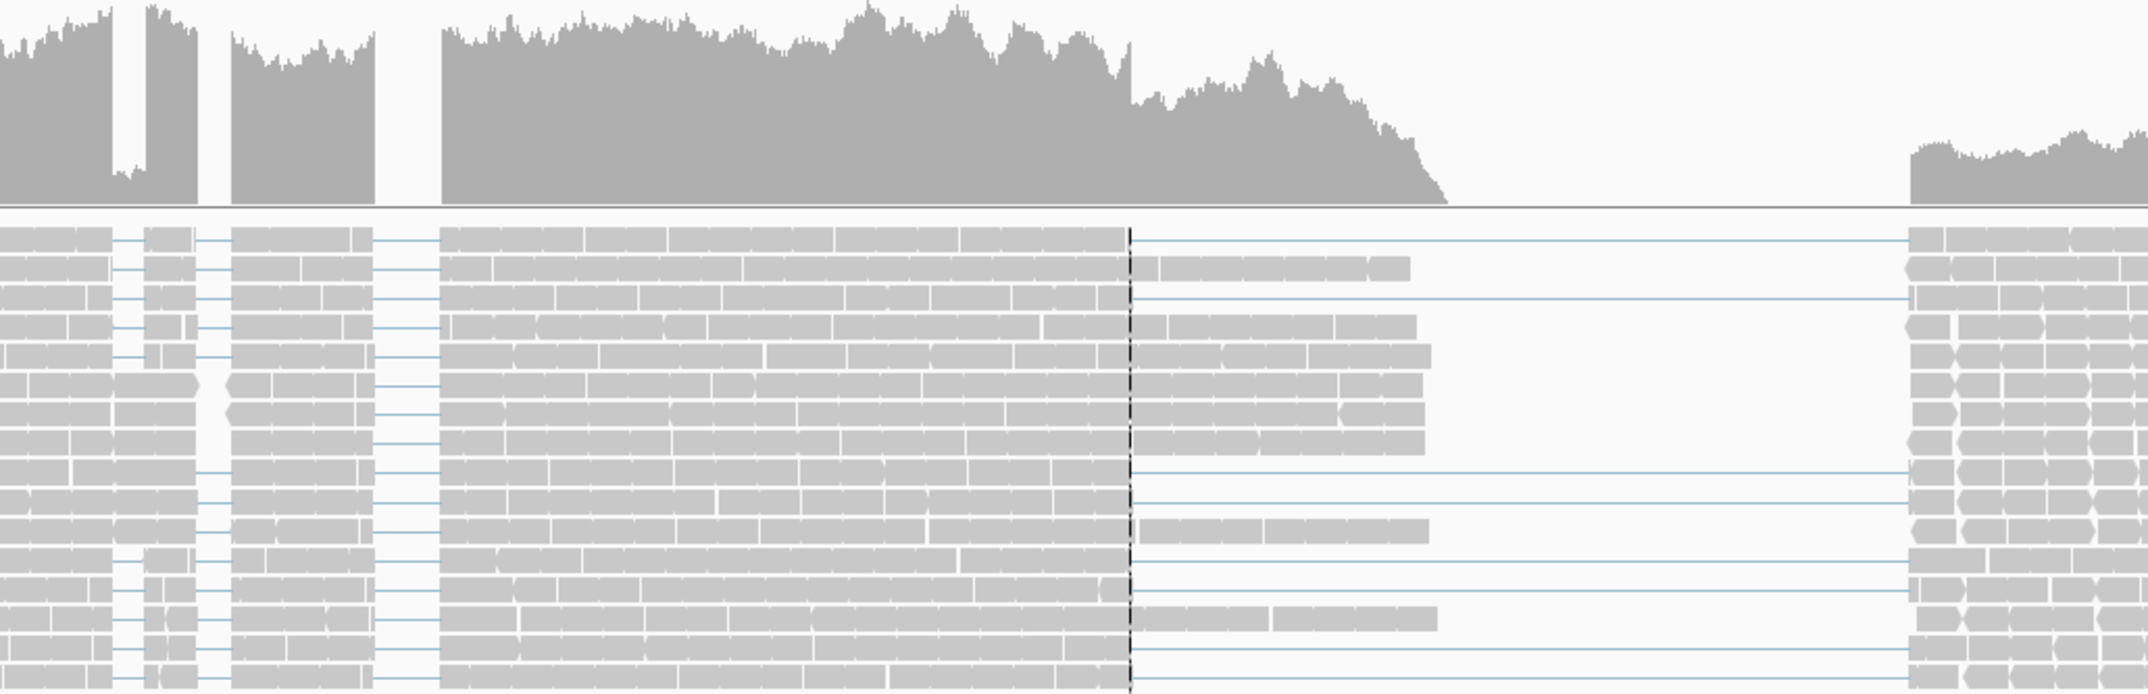
\includegraphics[width=\textwidth]{figures/reference.pdf}
	\vspace{0.2cm}
	\begin{center}

\begin{tikzpicture}[font=\small,overlay,
mycirclex/.style={draw, circle, minimum size=1.0em, inner sep = 0.2mm}, 
mydiamond/.style={draw, diamond, minimum size=0.78em, inner sep = 0mm}, 
myrectang/.style={draw, rectangle, minimum size=0.60em, inner sep = 0mm}, 
>=stealth]

\begin{scope}[xshift = -6cm, yshift=3.5cm]
\path<2-> node[blue] at (0.9cm, 0) {$1$};
\path<2-> node[blue] at (1.25cm, 0) {$2$};
\path<2-> node[blue] at (1.47cm,0) {$3$};
\path<2-> node[blue] at (2.1cm, 0) {$4$};
\path<2-> node[blue] at (4.5cm, 0) {$5$};
\path<2-> node[blue] at (7.0cm, 0) {$6$};
\path<2-> node[blue] at(10.8cm, 0) {$7$};
\end{scope}


\end{tikzpicture}
\end{center}

	\vspace{-0.4cm}
	\begin{center}

\begin{tikzpicture}[font=\small,overlay,
mycirclex/.style={draw, circle, minimum size=1.0em, inner sep = 0.2mm}, 
mydiamond/.style={draw, diamond, minimum size=0.78em, inner sep = 0mm}, 
myrectang/.style={draw, rectangle, minimum size=0.60em, inner sep = 0mm}, 
>=stealth]

\definecolor{mygreen}{rgb}{0, 0.7, 0}
\definecolor{myyellow}{rgb}{0.8, 0.6, 0}

\def\colx{black}
\def\cola{red} 
\def\colb{blue}
\def\colc{violet}
\def\cold{cyan} 
\def\cole{myyellow}
\def\colf{brown}


\def\len{2.0cm}

% G1
\begin{scope}[local bounding box=bbox, xshift=-6.0cm]
\path<1-> node[mycirclex] (v1) at (1.0 * \len, 0) {$s$};
\path<1-> node[mycirclex] (v2) at (2.0 * \len, 0) {$a$};
\path<1-> node[mycirclex] (v3) at (3.0 * \len, 0) {$b$};
\path<1-> node[mycirclex] (v4) at (4.0 * \len, 0) {$c$};
\path<1-> node[mycirclex] (v5) at (5.0 * \len, 0) {$t$};

\path<1-> [draw, \colx, ->, line width=0.04cm] (v1) -- (v2);
\path<1-> [draw, \colx, ->, line width=0.04cm] (v2) -- (v3);
\path<1-> [draw, \colx, ->, line width=0.04cm] (v3) -- (v4);
\path<1-> [draw, \colx, ->, line width=0.04cm] (v4) -- (v5);

\path<1-> [draw, \colx, ->, line width=0.04cm, bend left = 40] (v1) to (v3);
\path<1-> [draw, \colx, ->, line width=0.04cm, bend left = 40] (v3) to (v5);
\path<1-> [draw, \colx, ->, line width=0.04cm, bend left = 40] (v2) to (v4);

\path<1-> node at (1.5 * \len, 0.18cm) {$e_1(8)$};
\path<1-> node at (2.5 * \len, 0.18cm) {$e_2(2)$};
\path<1-> node at (3.5 * \len, 0.18cm) {$e_3(4)$};
\path<1-> node at (4.5 * \len, 0.18cm) {$e_4(10)$};

\path<1-> node at (2.0 * \len, 1.0cm) {$e_5(5)$};
\path<1-> node at (3.0 * \len, 1.0cm) {$e_6(6)$};
\path<1-> node at (4.0 * \len, 1.0cm) {$e_7(3)$};

\end{scope}
%\path<1-> [draw, rounded corners] ($(bbox.south west) - (0.00cm, 0.25cm)$) rectangle ($(bbox.north east) + (0.1cm, 0)$);
%\node at ($(bbox.south) - (0.00cm, 0.2cm)$) [label=below:{$G_2 - G_1 = \{c\}$}]{};


\end{tikzpicture}
\end{center}

	\vspace{0.2cm}
	\begin{itemize}
	\item<3-> {\bf Nodes:} continuous regions not seperated by spliced reads
	\item<3-> {\bf Edges:} two regions with spanning reads
	\item<4-> {\bf Weight of nodes:} estimated from the average coverage
	\item<4-> {\bf Weight of edges:} estimated from number of spanning reads
	\end{itemize}
}

\frame
{
	\frametitle{Optimization Problem}

	\begin{itemize}
	\item {\bf Input:} Directed acyclic graph~(DAG) $G=(V,E)$ with a single source $s$ and a single sink $t$;
		weight $w(e)$ for $e\in E$.

	\vspace{1.0cm}
	\begin{center}

\begin{tikzpicture}[font=\small,overlay,
mycirclex/.style={draw, circle, minimum size=1.0em, inner sep = 0.2mm}, 
mydiamond/.style={draw, diamond, minimum size=0.78em, inner sep = 0mm}, 
myrectang/.style={draw, rectangle, minimum size=0.60em, inner sep = 0mm}, 
>=stealth]

\definecolor{mygreen}{rgb}{0, 0.7, 0}
\definecolor{myyellow}{rgb}{0.8, 0.6, 0}

\def\colx{black}
\def\cola{red} 
\def\colb{blue}
\def\colc{violet}
\def\cold{cyan} 
\def\cole{myyellow}
\def\colf{brown}


\def\len{3.0cm}

% G1
\begin{scope}[local bounding box=bbox, xshift=-8.0cm]
\path<1-> node[mycirclex] (v1) at (1.0 * \len, 0) {$s$};
\path<1-> node[mycirclex] (v2) at (2.0 * \len, 0) {$a$};
\path<1-> node[mycirclex] (v3) at (3.0 * \len, 0) {$b$};
\path<1-> node[mycirclex] (v4) at (4.0 * \len, 0) {$t$};

\path<1-> [draw, \colc, ->, line width=0.04cm] (v1) -- (v2);
\path<1-> [draw, \colc, ->, line width=0.10cm, bend left = 40] (v2) to (v3);
\path<1-> [draw, \colc, ->, line width=0.10cm, bend left = 40] (v3) to (v4);

\path<1-> [draw, \colb, ->, line width=0.04cm] (v2) -- (v3);
\path<1-> [draw, \colb, ->, line width=0.10cm, bend left = 40] (v1) to (v2);
\path<1-> [draw, \colb, ->, line width=0.04cm, bend left = 40] (v3) to (v4);

\path<1-> [draw, \cola, ->, line width=0.04cm] (v3) -- (v4);
\path<1-> [draw, \cola, ->, line width=0.04cm, bend left = 40] (v1) to (v2);
\path<1-> [draw, \cola, ->, line width=0.04cm, bend left = 40] (v2) to (v3);


%\path<1-> [draw, \colx, ->, line width=0.02cm] (v1) -- (v2);
%\path<1-> [draw, \colx, ->, line width=0.02cm] (v2) -- (v3);
%\path<1-> [draw, \colx, ->, line width=0.02cm] (v3) -- (v4);
%
%\path<1-> [draw, \colx, ->, line width=0.02cm, bend left = 40] (v1) to (v2);
%\path<1-> [draw, \colx, ->, line width=0.02cm, bend left = 40] (v2) to (v3);
%\path<1-> [draw, \colx, ->, line width=0.02cm, bend left = 40] (v3) to (v4);

\path<1-> node at (1.5 * \len, 0.18cm) {$e_2(4)$};
\path<1-> node at (2.5 * \len, 0.18cm) {$e_4(3)$};
\path<1-> node at (3.5 * \len, 0.18cm) {$e_6(2)$};

\path<1-> node at (1.5 * \len, 0.85cm) {$e_1(5)$};
\path<1-> node at (2.5 * \len, 0.85cm) {$e_3(6)$};
\path<1-> node at (3.5 * \len, 0.85cm) {$e_5(7)$};

\end{scope}
%\path<1-> [draw, rounded corners] ($(bbox.south west) - (0.00cm, 0.25cm)$) rectangle ($(bbox.north east) + (0.1cm, 0)$);
%\node at ($(bbox.south) - (0.00cm, 0.2cm)$) [label=below:{$G_2 - G_1 = \{c\}$}]{};


\end{tikzpicture}
\end{center}

	\vspace{1.0cm}

	\vspace{0.5cm}

	\item<2-> {\bf Output:} A set of $s$-$t$ paths $\mathcal{P}$ and abundance $a(P)$ for $P\in\mathcal{P}$, such that
		\begin{enumerate}
		\vspace{0.1cm}
		\item each $e\in E$ is covered by at least one path $P\in\mathcal{P}$, and that
		\vspace{0.1cm}
		\item $|\mathcal{P}|$ is as small as possible, and that
		\vspace{0.1cm}
		\item $\sum_{e\in E} \|w(e) - \sum_{P:e\in P} a(P)\|$ is as small as possible.
		\end{enumerate}
	\end{itemize}

}

\frame
{
	\frametitle{Minimize the Number of Paths}
	{\bf Problem:} Given DAG $G=(V,E)$ with source $s$ and sink $t$, 
		to compute minimum number of paths that can cover all edges.

	\vspace{0.4cm}

	\begin{center}

\begin{tikzpicture}[font=\small,overlay,
mycirclex/.style={draw, circle, minimum size=1.0em, inner sep = 0.2mm}, 
mydiamond/.style={draw, diamond, minimum size=0.78em, inner sep = 0mm}, 
myrectang/.style={draw, rectangle, minimum size=0.60em, inner sep = 0mm}, 
>=stealth]

\definecolor{mygreen}{rgb}{0, 0.7, 0}
\definecolor{myyellow}{rgb}{0.8, 0.6, 0}

\def\colx{black}
\def\cola{red} 
\def\colb{blue}
\def\colc{violet}
\def\cold{cyan} 
\def\cole{myyellow}
\def\colf{brown}


\def\len{1.8cm}

% G1
\begin{scope}[local bounding box=bbox, xshift=-6.4cm]
\path<1-> node[mycirclex] (v1) at (1.0 * \len, 0) {$s$};
\path<1-> node[mycirclex] (v2) at (2.0 * \len, 0) {$a$};
\path<1-> node[mycirclex] (v3) at (3.0 * \len, 0) {$b$};
\path<1-> node[mycirclex] (v4) at (4.0 * \len, 0) {$c$};
\path<1-> node[mycirclex] (v5) at (5.0 * \len, 0) {$d$};

\path<1-> [draw, \colx, ->, line width=0.04cm] (v1) -- (v2);
\path<1-> [draw, \colx, ->, line width=0.04cm] (v2) -- (v3);
\path<1-> [draw, \colx, ->, line width=0.04cm] (v3) -- (v4);
\path<1-> [draw, \colx, ->, line width=0.04cm] (v4) -- (v5);

\path<1-> [draw, \colx, ->, line width=0.04cm, bend left = 40] (v1) to (v3);
\path<1-> [draw, \colx, ->, line width=0.04cm, bend left = 27] (v2) to (v5);
\path<1-> [draw, \colx, ->, line width=0.04cm, bend left =-40] (v2) to (v4);

\path<1-> node at (1.5 * \len, 0.18cm) {$e_1$};
\path<1-> node at (2.5 * \len, 0.18cm) {$e_2$};
\path<1-> node at (3.5 * \len, 0.18cm) {$e_3$};
\path<1-> node at (4.5 * \len, 0.18cm) {$e_4$};

\path<1-> node at (2.0 * \len, 0.9cm) {$e_5$};
\path<1-> node at (3.0 * \len,-0.6cm) {$e_6$};
\path<1-> node at (3.5 * \len, 0.9cm) {$e_7$};

\end{scope}
%\path<1-> [draw, rounded corners] ($(bbox.south west) - (0.00cm, 0.25cm)$) rectangle ($(bbox.north east) + (0.1cm, 0)$);
%\node at ($(bbox.south) - (0.00cm, 0.2cm)$) [label=below:{$G_2 - G_1 = \{c\}$}]{};


\end{tikzpicture}
\end{center}


	\vspace{0.6cm}

	\onslide<2->{{\bf Polynomial-time Algorithm:}}
	\vspace{-0.2cm}
	\begin{center}

\begin{tikzpicture}[font=\small,overlay,
mycirclex/.style={draw, circle, minimum size=1.0em, inner sep = 0.2mm}, 
mydiamond/.style={draw, diamond, minimum size=0.78em, inner sep = 0mm}, 
myrectang/.style={draw, rectangle, minimum size=0.60em, inner sep = 0mm}, 
>=stealth]

\definecolor{mygreen}{rgb}{0, 0.7, 0}
\definecolor{myyellow}{rgb}{0.8, 0.6, 0}

\def\colx{black}
\def\cola{red} 
\def\colb{blue}
\def\colc{violet}
\def\cold{cyan} 
\def\cole{myyellow}
\def\colf{brown}


\def\len{1.2cm}

% G1
\begin{scope}[local bounding box=bbox, xshift=-5.5cm]
\path<2-> node[mycirclex] (x1) at (1.0 * \len, 0.0) {$e_1$};
\path<2-> node[mycirclex] (x2) at (2.0 * \len, 0.0) {$e_2$};
\path<2-> node[mycirclex] (x3) at (3.0 * \len, 0.0) {$e_3$};
\path<2-> node[mycirclex] (x4) at (4.0 * \len, 0.0) {$e_4$};
\path<2-> node[mycirclex] (x5) at (5.0 * \len, 0.0) {$e_5$};
\path<2-> node[mycirclex] (x6) at (6.0 * \len, 0.0) {$e_6$};
\path<2-> node[mycirclex] (x7) at (7.0 * \len, 0.0) {$e_7$};

\path<2-> node[mycirclex] (y1) at (1.0 * \len, -2.0) {$e_1$};
\path<2-> node[mycirclex] (y2) at (2.0 * \len, -2.0) {$e_2$};
\path<2-> node[mycirclex] (y3) at (3.0 * \len, -2.0) {$e_3$};
\path<2-> node[mycirclex] (y4) at (4.0 * \len, -2.0) {$e_4$};
\path<2-> node[mycirclex] (y5) at (5.0 * \len, -2.0) {$e_5$};
\path<2-> node[mycirclex] (y6) at (6.0 * \len, -2.0) {$e_6$};
\path<2-> node[mycirclex] (y7) at (7.0 * \len, -2.0) {$e_7$};

\path<3-> [draw, \cola, line width=0.08cm] (x1) -- (y2);
\path<3-> [draw, \cola, line width=0.08cm] (x2) -- (y3);
\path<3-> [draw, \cola, line width=0.08cm] (x5) -- (y4);

\path<2-> [draw, \colx, line width=0.03cm] (x1) -- (y2);
\path<2-> [draw, \colx, line width=0.03cm] (x1) -- (y3);
\path<2-> [draw, \colx, line width=0.03cm] (x1) -- (y4);
\path<2-> [draw, \colx, line width=0.03cm] (x1) -- (y6);
\path<2-> [draw, \colx, line width=0.03cm] (x1) -- (y7);
\path<2-> [draw, \colx, line width=0.03cm] (x2) -- (y3);
\path<2-> [draw, \colx, line width=0.03cm] (x2) -- (y4);
\path<2-> [draw, \colx, line width=0.03cm] (x3) -- (y4);
\path<2-> [draw, \colx, line width=0.03cm] (x5) -- (y3);
\path<2-> [draw, \colx, line width=0.03cm] (x5) -- (y4);
\path<2-> [draw, \colx, line width=0.03cm] (x6) -- (y4);

\end{scope}
%\path<2-> [draw, rounded corners] ($(bbox.south west) - (0.00cm, 0.25cm)$) rectangle ($(bbox.north east) + (0.1cm, 0)$);
%\node at ($(bbox.south) - (0.00cm, 0.2cm)$) [label=below:{$G_2 - G_1 = \{c\}$}]{};


\end{tikzpicture}
\end{center}


	\vspace{2.0cm}
	\onslide<4->{{\bf Dilworth's Theorem:} $|\mathcal{P}| = |E| - M$.}
	
	\vspace{0.2cm}
	\onslide<5->{{\bf Existing Software:} Cufflinks~(Trapnell \emph{et al.}, 2010)}
}

\frame
{
	\frametitle{Minimize Abundance Error}
	{\bf Problem:} Given DAG $G=(V,E)$ with source $s$, sink $t$, and weight $w(e)$
	for $e\in E$, to compute a set of $s$-$t$ paths $\mathcal{P}$ so that all edges
	are covered and that $\sum_{e\in E} |w(e) - \sum_{P:e\in P} a(P)|$ is minimized.

	\vspace{0.2cm}
	\onslide<2->{{\bf Fact:} There exists a set of paths satisfying $x(e) = \sum_{P\in\mathcal{P}:e\in P} a(P)$ 
		for all $e\in E$ if and only if $x(e)$ forms a flow of $G$.}

	\vspace{0.2cm}
	\onslide<3->{{\bf Reformulation:} To compute $x(e)$ for $e\in E$ such that $x(e)$ forms a flow
		and that $\sum_{e\in E} |w(e) - x(e)|$ is minimized.}

	\vspace{0.2cm}
	\onslide<4->{{\bf Polynomial-time Algorithm}~(using LP):
	\begin{displaymath}
	\displaystyle
	\begin{array}{rl}
	\min & \sum_{e\in E} |w(e) - x(e)| \\
	\textrm{s.t.} & \left\{
		\begin{array}{ll}
			\sum_{e=(u,v)\in E} x(e) = \sum_{e=(v,w)\in E} x(e), \forall v \in V\\
			x(e) \ge 0, \forall e\in E
		\end{array}
		\right.
	\end{array}
	\end{displaymath}}

	\onslide<5->{Based on $x(e)$, {\bf greedy algorithm} can be used to retrieve $\mathcal{P}$
	with at most $|E| - |V| + 2$ paths.}

	\vspace{0.2cm}
	\onslide<6->{{\bf Existing Software:} Traph~(Tomescu \emph{et al.}, 2013)}
}

\frame
{
	\frametitle{Minimize Abundance Error with $k$ Paths}
	{\bf Problem:} Given DAG $G=(V,E)$ with source $s$, sink $t$, weight $w(e)$ for $e\in E$,
		to compute a set of at most $k$ $s$-$t$ paths $\mathcal{P}$ such that
			$\sum_{e\in E} \| w(e) - \sum_{P:e\in P} a(P)\|$ is minimized.

	\vspace{0.3cm}
	\onslide<2->{{\bf Maximum $k$-Splittable Flow Problem:} Given DAG $G=(V,E)$ with source
	$s$, sink $t$, weight $w(e)$ for $e\in E$, to compute a set of at most $k$
	$s$-$t$ paths $\mathcal{P}$ satisfying $\sum_{P:e\in P} a(P)\le w(e), \forall e\in E$~(capacity constraints) such that 
	$\sum_{P\in\mathcal{P}} a(P)$ is maximized.}

	\vspace{0.2cm}
	\begin{enumerate}
	\item<3-> {M$k$SF is {\bf NP}-hard for $2\le k < |E| - |V| + 2$.}
	\vspace{0.1cm}
	\item<4-> 1.5-approximation algorithm for $k=2$ and $k=3$.
	\vspace{0.1cm}
	\item<5-> 2-approximation algorithm for $4\le k < |E| - |V| + 2$.
	\vspace{0.1cm}
	\item<6-> Polynomial-time algorithm for $G$ with constant treewidth.
	\end{enumerate}
}

\frame
{
	\frametitle{Regularization Methods}

	{\bf Optimization Formulation:}
	\begin{displaymath}
	\min  \sum_{e\in E} \|w(e) - \sum_{P:e\in P} a(P)\| + \lambda \sum_{P\in\mathcal{P}} \|a(P)\|^q
	\end{displaymath}

	\vspace{0.2cm}
	\onslide<2->{
	\begin{enumerate}
	\item Initialize $\mathcal{P}$ as all possible paths~(exponential size).
	\item Parameter $\lambda$ needs to be trained.
	\item Use continuous optimization techniques~(Lasso, Newton–Raphson, etc) to compute a local optimal solution.
	\end{enumerate}}

	\vspace{0.2cm}
	\onslide<3->{{\bf Existing Softwares:} IsoLasso~(Li \emph{et al.}, 2011), SLIDE~(Li \emph{et al.}, 2011),
		CEM~(Li \emph{et al.}, 2012), MITIE~(Behr \emph{et al.}, 2013)}
}

\frame
{
	\frametitle{Heuristic---Greedy Algorithm}

	{\bf Algorithm:} Iteratively compute the path with maximum bottleneck weight, and then update the graph.
	\vspace{0.7cm}
	\begin{center}

\begin{tikzpicture}[font=\small,overlay,
mycirclex/.style={draw, circle, minimum size=1.0em, inner sep = 0.2mm}, 
mydiamond/.style={draw, diamond, minimum size=0.78em, inner sep = 0mm}, 
myrectang/.style={draw, rectangle, minimum size=0.60em, inner sep = 0mm}, 
>=stealth]

\definecolor{mygreen}{rgb}{0, 0.7, 0}
\definecolor{myyellow}{rgb}{0.8, 0.6, 0}

\def\colx{black}
\def\cola{red} 
\def\colb{blue}
\def\colc{violet}
\def\cold{cyan} 
\def\cole{myyellow}
\def\colf{brown}


\def\len{1.5cm}

% G1
\begin{scope}[local bounding box=bbox, xshift=-6cm]
\path<2-> node[mycirclex] (v1) at (1.0 * \len, 0) {$s$};
\path<2-> node[mycirclex] (v2) at (2.0 * \len, 0) {$a$};
\path<2-> node[mycirclex] (v3) at (3.0 * \len, 0) {$b$};
\path<2-> node[mycirclex] (v4) at (4.0 * \len, 0) {$c$};
\path<2-> node[mycirclex] (v5) at (5.0 * \len, 0) {$d$};
\path<2-> node[mycirclex] (v6) at (6.0 * \len, 0) {$t$};

\path<3-> [draw, \cola, ->, line width=0.09cm, bend left = 40] (v1) to (v3);
\path<3-> [draw, \cola, ->, line width=0.09cm] (v3) -- (v4);
\path<3-> [draw, \cola, ->, line width=0.09cm] (v4) -- (v5);
\path<3-> [draw, \cola, ->, line width=0.09cm] (v5) -- (v6);

\path<2-> [draw, \colx, ->, line width=0.04cm] (v1) -- (v2);
\path<2-> [draw, \colx, ->, line width=0.04cm] (v2) -- (v3);
\path<2-> [draw, \colx, ->, line width=0.04cm] (v3) -- (v4);
\path<2-> [draw, \colx, ->, line width=0.04cm] (v4) -- (v5);
\path<2-> [draw, \colx, ->, line width=0.04cm] (v5) -- (v6);

\path<2-> [draw, \colx, ->, line width=0.04cm, bend left = 40] (v1) to (v3);
\path<2-> [draw, \colx, ->, line width=0.04cm, bend left = 40] (v3) to (v5);
\path<2-> [draw, \colx, ->, line width=0.04cm, bend left =-27] (v2) to (v5);
\path<2-> [draw, \colx, ->, line width=0.04cm, bend left =-40] (v4) to (v6);

\path<2-> node at (1.5 * \len, 0.2cm) {$4$};
\path<2-> node at (2.5 * \len, 0.2cm) {$1$};
\path<2-> node at (3.5 * \len, 0.2cm) {$5$};
\path<2-> node at (4.5 * \len, 0.2cm) {$4$};
\path<2-> node at (5.5 * \len, 0.2cm) {$9$};

\path<2-> node at (2.0 * \len, 0.85cm) {$6$};
\path<2-> node at (4.0 * \len, 0.85cm) {$2$};
\path<2-> node at (5.0 * \len,-0.85cm) {$1$};
\path<2-> node at (3.5 * \len,-0.85cm) {$3$};

\path<4-> [draw, \colx, ->, line width=0.1cm] (3.5 * \len, -1.2cm) -- (3.5 * \len, -1.8cm);

\end{scope}

%\path<2-> [draw, rounded corners] ($(bbox.south west) - (0.00cm, 0.25cm)$) rectangle ($(bbox.north east) + (0.1cm, 0)$);
%\node at ($(bbox.south) - (0.00cm, 0.2cm)$) [label=below:{$G_2 - G_1 = \{c\}$}]{};


% G2
\begin{scope}[local bounding box=bbox, xshift=-6cm, yshift = -2.6cm]
\path<4-> node[mycirclex] (v1) at (1.0 * \len, 0) {$s$};
\path<4-> node[mycirclex] (v2) at (2.0 * \len, 0) {$a$};
\path<4-> node[mycirclex] (v3) at (3.0 * \len, 0) {$b$};
\path<4-> node[mycirclex] (v4) at (4.0 * \len, 0) {$c$};
\path<4-> node[mycirclex] (v5) at (5.0 * \len, 0) {$d$};
\path<4-> node[mycirclex] (v6) at (6.0 * \len, 0) {$t$};

\path<4-> [draw, \colx, ->, line width=0.04cm] (v1) -- (v2);
\path<4-> [draw, \colx, ->, line width=0.04cm] (v2) -- (v3);
\path<4-> [draw, \colx, ->, line width=0.04cm] (v3) -- (v4);
\path<4-> [draw, \colx, ->, line width=0.04cm] (v5) -- (v6);

\path<4-> [draw, \colx, ->, line width=0.04cm, bend left = 40] (v1) to (v3);
\path<4-> [draw, \colx, ->, line width=0.04cm, bend left = 40] (v3) to (v5);
\path<4-> [draw, \colx, ->, line width=0.04cm, bend left =-27] (v2) to (v5);
\path<4-> [draw, \colx, ->, line width=0.04cm, bend left =-40] (v4) to (v6);

\path<4-> node at (1.5 * \len, 0.2cm) {$4$};
\path<4-> node at (2.5 * \len, 0.2cm) {$1$};
\path<4-> node at (3.5 * \len, 0.2cm) {$1$};
\path<4-> node at (5.5 * \len, 0.2cm) {$5$};

\path<4-> node at (2.0 * \len, 0.85cm) {$2$};
\path<4-> node at (4.0 * \len, 0.85cm) {$2$};
\path<4-> node at (5.0 * \len,-0.85cm) {$1$};
\path<4-> node at (3.5 * \len,-0.85cm) {$3$};
\end{scope}


\end{tikzpicture}
\end{center}

	\vspace{3.5cm}
	\onslide<6->{{\bf Existing Softwares:} Traph~(Tomescu \emph{et al.}, 2013), StringTie~(Pertea \emph{et al.}, 2015)}
}

\frame
{
	\frametitle{Our Method}
	\begin{enumerate}
	\item Initialize a set of paths $\mathcal{P}$~(in polynomial size).
	\vspace{0.2cm}
	\item Use LP to estimate the abundance of the paths in $\mathcal{B}$ to minimize the estimation error.
	\vspace{0.2cm}
	\item Reduce the number of paths in $\mathcal{P}$:
		\begin{itemize}
		\vspace{0.1cm}
		\item For two paths with (almost) identical abundance, try to merge them into one path;
		\vspace{0.1cm}
		\item Discard paths with very small abundance.
		\end{itemize}
	\vspace{0.2cm}
	\item Iterate between step 2 and step 3.
	\end{enumerate}
}

\frame
{
	\frametitle{Bad Example for Greedy Algorithm}

	\vspace{0.2cm}
	\begin{center}

\begin{tikzpicture}[font=\small,overlay,
mycirclex/.style={draw, circle, minimum size=1.0em, inner sep = 0.2mm}, 
mydiamond/.style={draw, diamond, minimum size=0.78em, inner sep = 0mm}, 
myrectang/.style={draw, rectangle, minimum size=0.60em, inner sep = 0mm}, 
>=stealth]

\definecolor{mygreen}{rgb}{0, 0.7, 0}
\definecolor{myyellow}{rgb}{0.8, 0.6, 0}

\def\colx{black}
\def\cola{red} 
\def\colb{blue}
\def\colc{violet}
\def\cold{cyan} 
\def\cole{myyellow}
\def\colf{brown}


\def\len{1.8cm}

% G1
\begin{scope}[local bounding box=bbox, xshift=-6.4cm, yscale=1.2]
\path<2-> node[mycirclex] (v1) at (1.0 * \len, 0) {$s$};
\path<2-> node[mycirclex] (v2) at (2.0 * \len, 0) {$a$};
\path<2-> node[mycirclex] (v3) at (3.0 * \len, 0) {$b$};
\path<2-> node[mycirclex] (v4) at (4.0 * \len, 0) {$c$};
\path<2-> node[mycirclex] (v5) at (5.0 * \len, 0) {$d$};
\path<2-> node[mycirclex] (v6) at (6.0 * \len, 0) {$t$};

\path<3-> [draw, opacity = 1.0, \cola, ->, line width=0.082cm] (v1) -- (v2);
\path<3-> [draw, opacity = 1.0, \cola, ->, line width=0.082cm] (v2) -- (v3);
\path<3-> [draw, opacity = 1.0, \cola, ->, line width=0.082cm] (v3) -- (v4);
\path<3-> [draw, opacity = 1.0, \cola, ->, line width=0.082cm] (v4) -- (v5);
\path<3-> [draw, opacity = 1.0, \cola, ->, line width=0.082cm] (v5) -- (v6);
\path<4-> [draw, \colb, opacity = 1.0, ->, line width=0.082cm, bend left = 50] (v1) to (v2);
\path<4-> [draw, \colb, opacity = 1.0, ->, line width=0.082cm, bend left = 30] (v3) to (v6);
\path<4-> [draw, \colb, opacity = 1.0, ->, line width=0.082cm, bend left =-20] (v2) to (v3);
\path<5-> [draw, \colc, opacity = 1.0, ->, line width=0.082cm, bend left = 50] (v5) to (v6);
\path<5-> [draw, \colc, opacity = 1.0, ->, line width=0.082cm, bend left = 30] (v1) to (v4);
\path<5-> [draw, \colc, opacity = 1.0, ->, line width=0.082cm, bend left =-20] (v4) to (v5);

\path<2-> [draw, \colx, ->, line width=0.02cm] (v1) -- (v2);
\path<2-> [draw, \colx, ->, line width=0.02cm] (v2) -- (v3);
\path<2-> [draw, \colx, ->, line width=0.02cm] (v3) -- (v4);
\path<2-> [draw, \colx, ->, line width=0.02cm] (v4) -- (v5);
\path<2-> [draw, \colx, ->, line width=0.02cm] (v5) -- (v6);

\path<2-> [draw, \colx, ->, line width=0.02cm, bend left = 50] (v1) to (v2);
\path<2-> [draw, \colx, ->, line width=0.02cm, bend left = 50] (v5) to (v6);
\path<2-> [draw, \colx, ->, line width=0.02cm, bend left = 30] (v1) to (v4);
\path<2-> [draw, \colx, ->, line width=0.02cm, bend left = 30] (v3) to (v6);

\path<2-> [draw, \colx, ->, line width=0.02cm, bend left =-20] (v2) to (v3);
\path<2-> [draw, \colx, ->, line width=0.02cm, bend left =-30] (v2) to (v3);
\path<2-> [draw, \colx, ->, line width=0.02cm, bend left =-40] (v2) to (v3);
\path<2-> [draw, \colx, ->, line width=0.02cm, bend left =-50] (v2) to (v3);
\path<2-> [draw, \colx, ->, line width=0.02cm, bend left =-20] (v4) to (v5);
\path<2-> [draw, \colx, ->, line width=0.02cm, bend left =-30] (v4) to (v5);
\path<2-> [draw, \colx, ->, line width=0.02cm, bend left =-40] (v4) to (v5);
\path<2-> [draw, \colx, ->, line width=0.02cm, bend left =-50] (v4) to (v5);


\path<2-> node at (1.5 * \len, 0.17cm) {$2n$};
\path<2-> node at (2.5 * \len, 0.17cm) {$2n$};
\path<2-> node at (3.5 * \len, 0.17cm) {$2n$};
\path<2-> node at (4.5 * \len, 0.17cm) {$2n$};
\path<2-> node at (5.5 * \len, 0.17cm) {$2n$};

\path<2-> node at (1.4 * \len, 0.62cm) {$n$};
\path<2-> node at (5.6 * \len, 0.62cm) {$n$};
\path<2-> node at (2.5 * \len, 0.96cm) {$n$};
\path<2-> node at (4.5 * \len, 0.96cm) {$n$};

\path<2-> node at (2.5 * \len, -0.65cm) {$n\times 1$};
\path<2-> node at (4.5 * \len, -0.65cm) {$n\times 1$};
\end{scope}


\end{tikzpicture}
\end{center}

	\vspace{0.8cm}
	\onslide<6->{{\bf Solution by greedy algorithm:} $2n + 1$ paths.}

	\vspace{1.5cm}
	\begin{center}


\begin{tikzpicture}[font=\small,overlay,
mycirclex/.style={draw, circle, minimum size=1.0em, inner sep = 0.2mm}, 
mydiamond/.style={draw, diamond, minimum size=0.78em, inner sep = 0mm}, 
myrectang/.style={rounded corners, draw, rectangle, minimum size=0.60em, inner sep = 0.8mm, line width = 0.03cm}, 
>=stealth]

\definecolor{mygreen}{rgb}{0, 0.7, 0}
\definecolor{myyellow}{rgb}{0.8, 0.6, 0}

\def\colx{black}
\def\cola{red} 
\def\colb{blue}
\def\colc{violet}
\def\cold{cyan} 
\def\cole{myyellow}
\def\colf{brown}


\def\len{1.65cm}

% G1
\begin{scope}[local bounding box=bbox, xshift=-6.9cm, yscale=1.2]
\path<7-> node[mycirclex] (v1) at (1.0 * \len, 0) {$s$};
\path<7-> node[mycirclex] (v2) at (2.0 * \len, 0) {$a$};
\path<7-> node[mycirclex] (v3) at (3.0 * \len, 0) {$b$};
\path<7-> node[mycirclex] (v4) at (4.0 * \len, 0) {$c$};
\path<7-> node[mycirclex] (v5) at (5.0 * \len, 0) {$d$};
\path<7-> node[mycirclex] (v6) at (6.0 * \len, 0) {$t$};

\path<11-> [draw, \cold, ->, line width=0.122cm, bend left = 50] (v1) to (v2);
\path<11-> [draw, \cold, ->, line width=0.122cm, bend left =-20] (v2) to (v3);
\path<11-> [draw, \cold, ->, line width=0.122cm, bend left =-20] (v4) to (v5);
\path<11-> [draw, \cold, ->, line width=0.122cm, bend left = 50] (v5) to (v6);
\path<11-> [draw, \cold, ->, line width=0.122cm] (v3) -- (v4);
\path<11-> node[myrectang, rounded corners, \cold] at (7 * \len, -0.75cm) {$a(P_4) = 1~(\times n)$};

\path<10-> [draw, \colc, ->, line width=0.122cm, bend left = 30] (v1) to (v4);
\path<10-> [draw, \colc, ->, line width=0.122cm] (v4) -- (v5);
\path<10-> [draw, \colc, ->, line width=0.122cm] (v5) -- (v6);
\path<10-> node[myrectang, rounded corners, \colc] at (7 * \len, -0.25cm) {$a(P_3) = n~(\times 1)$};

\path<9-> [draw, \colb, ->, line width=0.122cm] (v1) -- (v2);
\path<9-> [draw, \colb, ->, line width=0.122cm] (v2) -- (v3);
\path<9-> [draw, \colb, ->, line width=0.122cm, bend left = 30] (v3) to (v6);
\path<9-> node[myrectang, rounded corners, \colb] at (7 * \len, 0.25cm) {$a(P_2) = n~(\times 1)$};


\path<8-> [draw, \cola, ->, line width=0.052cm] (v1) -- (v2);
\path<8-> [draw, \cola, ->, line width=0.052cm] (v2) -- (v3);
\path<8-> [draw, \cola, ->, line width=0.052cm] (v3) -- (v4);
\path<8-> [draw, \cola, ->, line width=0.052cm] (v4) -- (v5);
\path<8-> [draw, \cola, ->, line width=0.052cm] (v5) -- (v6);
\path<8-> node[myrectang, rounded corners, \cola] at (7 * \len, 0.75cm) {$a(P_1) = n~(\times 1)$};

\path<7-> [draw, \colx, ->, line width=0.02cm] (v1) -- (v2);
\path<7-> [draw, \colx, ->, line width=0.02cm] (v2) -- (v3);
\path<7-> [draw, \colx, ->, line width=0.02cm] (v3) -- (v4);
\path<7-> [draw, \colx, ->, line width=0.02cm] (v4) -- (v5);
\path<7-> [draw, \colx, ->, line width=0.02cm] (v5) -- (v6);

\path<7-> [draw, \colx, ->, line width=0.02cm, bend left = 50] (v1) to (v2);
\path<7-> [draw, \colx, ->, line width=0.02cm, bend left = 50] (v5) to (v6);
\path<7-> [draw, \colx, ->, line width=0.02cm, bend left = 30] (v1) to (v4);
\path<7-> [draw, \colx, ->, line width=0.02cm, bend left = 30] (v3) to (v6);

\path<7-> [draw, \colx, ->, line width=0.02cm, bend left =-20] (v2) to (v3);
\path<7-> [draw, \colx, ->, line width=0.02cm, bend left =-30] (v2) to (v3);
\path<7-> [draw, \colx, ->, line width=0.02cm, bend left =-40] (v2) to (v3);
\path<7-> [draw, \colx, ->, line width=0.02cm, bend left =-50] (v2) to (v3);
\path<7-> [draw, \colx, ->, line width=0.02cm, bend left =-20] (v4) to (v5);
\path<7-> [draw, \colx, ->, line width=0.02cm, bend left =-30] (v4) to (v5);
\path<7-> [draw, \colx, ->, line width=0.02cm, bend left =-40] (v4) to (v5);
\path<7-> [draw, \colx, ->, line width=0.02cm, bend left =-50] (v4) to (v5);


\path<7-> node at (1.5 * \len, 0.17cm) {$2n$};
\path<7-> node at (2.5 * \len, 0.17cm) {$2n$};
\path<7-> node at (3.5 * \len, 0.17cm) {$2n$};
\path<7-> node at (4.5 * \len, 0.17cm) {$2n$};
\path<7-> node at (5.5 * \len, 0.17cm) {$2n$};

\path<7-> node at (1.4 * \len, 0.62cm) {$n$};
\path<7-> node at (5.6 * \len, 0.62cm) {$n$};
\path<7-> node at (2.5 * \len, 0.96cm) {$n$};
\path<7-> node at (4.5 * \len, 0.96cm) {$n$};

\path<7-> node at (2.5 * \len, -0.65cm) {$n\times 1$};
\path<7-> node at (4.5 * \len, -0.65cm) {$n\times 1$};
\end{scope}


\end{tikzpicture}
\end{center}

	\vspace{0.8cm}
	\onslide<12->{{\bf Optimal solution:} $n + 3$ paths.}
}

\frame
{
	\frametitle{Use the Residual Graph}

	\vspace{-3.4cm}
	\begin{center}

\begin{tikzpicture}[font=\small,overlay,
mycirclex/.style={draw, circle, minimum size=1.0em, inner sep = 0.2mm}, 
mydiamond/.style={draw, diamond, minimum size=0.78em, inner sep = 0mm}, 
myrectang/.style={rounded corners, draw, rectangle, minimum size=0.60em, inner sep = 0.8mm, line width = 0.03cm}, 
>=stealth]

\definecolor{mygreen}{rgb}{0, 0.7, 0}
\definecolor{myyellow}{rgb}{0.8, 0.6, 0}

\def\colx{black}
\def\cola{red} 
\def\colb{blue}
\def\colc{violet}
\def\cold{cyan} 
\def\cole{myyellow}
\def\colf{brown}


\def\len{1.65cm}

% G1
\begin{scope}[local bounding box=bbox, xshift=-6.9cm, yscale=1.2]
\path<2-> node[mycirclex] (v1) at (1.0 * \len, 0) {$s$};
\path<2-> node[mycirclex] (v2) at (2.0 * \len, 0) {$a$};
\path<2-> node[mycirclex] (v3) at (3.0 * \len, 0) {$b$};
\path<2-> node[mycirclex] (v4) at (4.0 * \len, 0) {$c$};
\path<2-> node[mycirclex] (v5) at (5.0 * \len, 0) {$d$};
\path<2-> node[mycirclex] (v6) at (6.0 * \len, 0) {$t$};

\path<3-> [draw, opacity = 1.0, \cola, ->, line width=0.082cm] (v1) -- (v2);
\path<3-> [draw, opacity = 1.0, \cola, ->, line width=0.082cm] (v2) -- (v3);
\path<3-> [draw, opacity = 1.0, \cola, ->, line width=0.082cm] (v3) -- (v4);
\path<3-> [draw, opacity = 1.0, \cola, ->, line width=0.082cm] (v4) -- (v5);
\path<3-> [draw, opacity = 1.0, \cola, ->, line width=0.082cm] (v5) -- (v6);
\path<3-> node[myrectang, rounded corners, \cola] at (7.03 * \len, 0.0cm) {$a(P_1) = 2n~(\times 1)$};

\path<2-> [draw, \colx, ->, line width=0.02cm] (v1) -- (v2);
\path<2-> [draw, \colx, ->, line width=0.02cm] (v2) -- (v3);
\path<2-> [draw, \colx, ->, line width=0.02cm] (v3) -- (v4);
\path<2-> [draw, \colx, ->, line width=0.02cm] (v4) -- (v5);
\path<2-> [draw, \colx, ->, line width=0.02cm] (v5) -- (v6);

\path<2-> [draw, \colx, ->, line width=0.02cm, bend left = 50] (v1) to (v2);
\path<2-> [draw, \colx, ->, line width=0.02cm, bend left = 50] (v5) to (v6);
\path<2-> [draw, \colx, ->, line width=0.02cm, bend left = 30] (v1) to (v4);
\path<2-> [draw, \colx, ->, line width=0.02cm, bend left = 30] (v3) to (v6);

\path<2-> [draw, \colx, ->, line width=0.02cm, bend left =-20] (v2) to (v3);
\path<2-> [draw, \colx, ->, line width=0.02cm, bend left =-30] (v2) to (v3);
\path<2-> [draw, \colx, ->, line width=0.02cm, bend left =-40] (v2) to (v3);
\path<2-> [draw, \colx, ->, line width=0.02cm, bend left =-50] (v2) to (v3);
\path<2-> [draw, \colx, ->, line width=0.02cm, bend left =-20] (v4) to (v5);
\path<2-> [draw, \colx, ->, line width=0.02cm, bend left =-30] (v4) to (v5);
\path<2-> [draw, \colx, ->, line width=0.02cm, bend left =-40] (v4) to (v5);
\path<2-> [draw, \colx, ->, line width=0.02cm, bend left =-50] (v4) to (v5);


\path<2-> node at (1.5 * \len, 0.17cm) {$2n$};
\path<2-> node at (2.5 * \len, 0.17cm) {$2n$};
\path<2-> node at (3.5 * \len, 0.17cm) {$2n$};
\path<2-> node at (4.5 * \len, 0.17cm) {$2n$};
\path<2-> node at (5.5 * \len, 0.17cm) {$2n$};

\path<2-> node at (1.4 * \len, 0.62cm) {$n$};
\path<2-> node at (5.6 * \len, 0.62cm) {$n$};
\path<2-> node at (2.5 * \len, 0.96cm) {$n$};
\path<2-> node at (4.5 * \len, 0.96cm) {$n$};

\path<2-> node at (2.5 * \len, -0.65cm) {$n\times 1$};
\path<2-> node at (4.5 * \len, -0.65cm) {$n\times 1$};

\path<4-> [draw, line width = 0.1cm, ->] (3.5 * \len, -0.7cm) to node[label=right:{Residual Graph}]{} (3.5 * \len, -1.4cm);
\end{scope}

% G2
\begin{scope}[local bounding box=bbox, xshift=-6.9cm, yscale=1.2, yshift=-2.4cm]
\path<4-> node[mycirclex] (v1) at (1.0 * \len, 0) {$s$};
\path<4-> node[mycirclex] (v2) at (2.0 * \len, 0) {$a$};
\path<4-> node[mycirclex] (v3) at (3.0 * \len, 0) {$b$};
\path<4-> node[mycirclex] (v4) at (4.0 * \len, 0) {$c$};
\path<4-> node[mycirclex] (v5) at (5.0 * \len, 0) {$d$};
\path<4-> node[mycirclex] (v6) at (6.0 * \len, 0) {$t$};

\path<5-> [draw, \colb, opacity = 1.0, ->, line width=0.082cm, bend left = 30] (v1) to (v4);
\path<5-> [draw, \colb, opacity = 1.0, <-, line width=0.082cm] (v3) -- (v4);
\path<5-> [draw, \colb, opacity = 1.0, ->, line width=0.082cm, bend left = 30] (v3) to (v6);
\path<5-> node[myrectang, rounded corners, \colb] at (7.03 * \len, 0.0cm) {$a(P_2) = n~(\times 1)$};

\path<4-> [draw, \colx, <-, line width=0.02cm] (v1) -- (v2);
\path<4-> [draw, \colx, <-, line width=0.02cm] (v2) -- (v3);
\path<4-> [draw, \colx, <-, line width=0.02cm] (v3) -- (v4);
\path<4-> [draw, \colx, <-, line width=0.02cm] (v4) -- (v5);
\path<4-> [draw, \colx, <-, line width=0.02cm] (v5) -- (v6);

\path<4-> [draw, \colx, ->, line width=0.02cm, bend left = 50] (v1) to (v2);
\path<4-> [draw, \colx, ->, line width=0.02cm, bend left = 50] (v5) to (v6);
\path<4-> [draw, \colx, ->, line width=0.02cm, bend left = 30] (v1) to (v4);
\path<4-> [draw, \colx, ->, line width=0.02cm, bend left = 30] (v3) to (v6);

\path<4-> [draw, \colx, ->, line width=0.02cm, bend left =-20] (v2) to (v3);
\path<4-> [draw, \colx, ->, line width=0.02cm, bend left =-30] (v2) to (v3);
\path<4-> [draw, \colx, ->, line width=0.02cm, bend left =-40] (v2) to (v3);
\path<4-> [draw, \colx, ->, line width=0.02cm, bend left =-50] (v2) to (v3);
\path<4-> [draw, \colx, ->, line width=0.02cm, bend left =-20] (v4) to (v5);
\path<4-> [draw, \colx, ->, line width=0.02cm, bend left =-30] (v4) to (v5);
\path<4-> [draw, \colx, ->, line width=0.02cm, bend left =-40] (v4) to (v5);
\path<4-> [draw, \colx, ->, line width=0.02cm, bend left =-50] (v4) to (v5);


\path<4-> node at (1.5 * \len, 0.17cm) {$2n$};
\path<4-> node at (2.5 * \len, 0.17cm) {$2n$};
\path<4-> node at (3.5 * \len, 0.17cm) {$2n$};
\path<4-> node at (4.5 * \len, 0.17cm) {$2n$};
\path<4-> node at (5.5 * \len, 0.17cm) {$2n$};

\path<4-> node at (1.4 * \len, 0.62cm) {$n$};
\path<4-> node at (5.6 * \len, 0.62cm) {$n$};
\path<4-> node at (2.5 * \len, 0.96cm) {$n$};
\path<4-> node at (4.5 * \len, 0.96cm) {$n$};

\path<4-> node at (2.5 * \len, -0.65cm) {$n\times 1$};
\path<4-> node at (4.5 * \len, -0.65cm) {$n\times 1$};
\path<6-> [draw, line width = 0.1cm, ->] (3.5 * \len, -0.7cm) to node[label=right:{Residual Graph}]{} (3.5 * \len, -1.4cm);
\end{scope}

% G3
\begin{scope}[local bounding box=bbox, xshift=-6.9cm, yscale=1.2, yshift=-4.8cm]
\path<6-> node[mycirclex] (v1) at (1.0 * \len, 0) {$s$};
\path<6-> node[mycirclex] (v2) at (2.0 * \len, 0) {$a$};
\path<6-> node[mycirclex] (v3) at (3.0 * \len, 0) {$b$};
\path<6-> node[mycirclex] (v4) at (4.0 * \len, 0) {$c$};
\path<6-> node[mycirclex] (v5) at (5.0 * \len, 0) {$d$};
\path<6-> node[mycirclex] (v6) at (6.0 * \len, 0) {$t$};

\path<7-> [draw, \cold, ->, line width=0.082cm, bend left = 50] (v1) to (v2);
\path<7-> [draw, \cold, ->, line width=0.082cm, bend left =-20] (v2) to (v3);
\path<7-> [draw, \cold, ->, line width=0.082cm, bend left = 10] (v3) to (v4);
\path<7-> [draw, \cold, ->, line width=0.082cm, bend left =-20] (v4) to (v5);
\path<7-> [draw, \cold, ->, line width=0.082cm, bend left = 50] (v5) to (v6);
\path<7-> node[myrectang, rounded corners, \cold] at (7.03 * \len, 0.0cm) {$a(P_3) = 1~(\times n)$};

\path<6-> [draw, \colx, <-, line width=0.02cm] (v1) -- (v2);
\path<6-> [draw, \colx, <-, line width=0.02cm] (v2) -- (v3);
\path<6-> [draw, \colx, <-, line width=0.02cm] (v4) -- (v5);
\path<6-> [draw, \colx, <-, line width=0.02cm] (v5) -- (v6);

\path<6-> [draw, \colx, ->, line width=0.02cm, bend left = 10] (v3) to (v4);
\path<6-> [draw, \colx, <-, line width=0.02cm, bend left =-10] (v3) to (v4);

\path<6-> [draw, \colx, ->, line width=0.02cm, bend left = 50] (v1) to (v2);
\path<6-> [draw, \colx, ->, line width=0.02cm, bend left = 50] (v5) to (v6);
\path<6-> [draw, \colx, <-, line width=0.02cm, bend left = 30] (v1) to (v4);
\path<6-> [draw, \colx, <-, line width=0.02cm, bend left = 30] (v3) to (v6);

\path<6-> [draw, \colx, ->, line width=0.02cm, bend left =-20] (v2) to (v3);
\path<6-> [draw, \colx, ->, line width=0.02cm, bend left =-30] (v2) to (v3);
\path<6-> [draw, \colx, ->, line width=0.02cm, bend left =-40] (v2) to (v3);
\path<6-> [draw, \colx, ->, line width=0.02cm, bend left =-50] (v2) to (v3);
\path<6-> [draw, \colx, ->, line width=0.02cm, bend left =-20] (v4) to (v5);
\path<6-> [draw, \colx, ->, line width=0.02cm, bend left =-30] (v4) to (v5);
\path<6-> [draw, \colx, ->, line width=0.02cm, bend left =-40] (v4) to (v5);
\path<6-> [draw, \colx, ->, line width=0.02cm, bend left =-50] (v4) to (v5);


\path<6-> node at (1.5 * \len, 0.17cm) {$2n$};
\path<6-> node at (2.5 * \len, 0.17cm) {$2n$};
\path<6-> node at (4.5 * \len, 0.17cm) {$2n$};
\path<6-> node at (5.5 * \len, 0.17cm) {$2n$};

\path<6-> node at (3.5 * \len, 0.2cm) {$n$};
\path<6-> node at (3.5 * \len, -0.2cm) {$n$};

\path<6-> node at (1.4 * \len, 0.62cm) {$n$};
\path<6-> node at (5.6 * \len, 0.62cm) {$n$};
\path<6-> node at (2.5 * \len, 0.96cm) {$n$};
\path<6-> node at (4.5 * \len, 0.96cm) {$n$};

\path<6-> node at (2.5 * \len, -0.65cm) {$n\times 1$};
\path<6-> node at (4.5 * \len, -0.65cm) {$n\times 1$};
\end{scope}



\end{tikzpicture}
\end{center}

	%\onslide<5->{Compute the maximum bottleneck path in the {\bf residual graph}.}
}

\frame
{
	\frametitle{Resolve Path with Backward Edges}

	\vspace{0.2cm}
	\begin{center}


\begin{tikzpicture}[font=\small,overlay,
mycirclex/.style={draw, circle, minimum size=1.0em, inner sep = 0.2mm}, 
mydiamond/.style={draw, diamond, minimum size=0.78em, inner sep = 0mm}, 
myrectang/.style={draw, rectangle, minimum size=0.60em, inner sep = 0mm}, 
>=stealth]

\definecolor{mygreen}{rgb}{0, 0.7, 0}
\definecolor{myyellow}{rgb}{0.8, 0.6, 0}

\def\colx{black}
\def\cola{red} 
\def\colb{blue}
\def\colc{violet}
\def\cold{cyan} 
\def\cole{myyellow}
\def\colf{brown}


\def\len{1.8cm}

% G1
\begin{scope}[local bounding box=bbox, xshift=-6.4cm, yscale=1.2]
\path<2-> node[mycirclex] (v1) at (1.0 * \len, 0) {$s$};
\path<2-> node[mycirclex] (v2) at (2.0 * \len, 0) {$a$};
\path<2-> node[mycirclex] (v3) at (3.0 * \len, 0) {$b$};
\path<2-> node[mycirclex] (v4) at (4.0 * \len, 0) {$c$};
\path<2-> node[mycirclex] (v5) at (5.0 * \len, 0) {$d$};
\path<2-> node[mycirclex] (v6) at (6.0 * \len, 0) {$t$};

\path<3-> [draw, \colb, ->, line width=0.10cm, bend left = 30] (v1) to (v4);
\path<3-> [draw, \colb, ->, line width=0.10cm, bend left = 30] (v3) to (v6);
\path<3-3> [draw, \colb, <-, line width=0.10cm] (v3) -- (v4);

\path<2-> [draw, \cola, ->, line width=0.05cm] (v1) -- (v2);
\path<2-> [draw, \cola, ->, line width=0.05cm] (v2) -- (v3);
\path<2-3> [draw, \cola, ->, line width=0.05cm] (v3) -- (v4);
\path<2-> [draw, \cola, ->, line width=0.05cm] (v4) -- (v5);
\path<2-> [draw, \cola, ->, line width=0.05cm] (v5) -- (v6);

\path<5-> [draw, line width = 0.1cm, ->] (3.5 * \len, -0.8cm) to node[label=right:{resolved}]{} (3.5 * \len, -1.7cm);
\end{scope}

% G2
\begin{scope}[local bounding box=bbox, xshift=-6.4cm, yscale=1.2, yshift=-3.0cm]
\path<5-> node[mycirclex] (v1) at (1.0 * \len, 0) {$s$};
\path<5-> node[mycirclex] (v2) at (2.0 * \len, 0) {$a$};
\path<5-> node[mycirclex] (v3) at (3.0 * \len, 0) {$b$};
\path<5-> node[mycirclex] (v4) at (4.0 * \len, 0) {$c$};
\path<5-> node[mycirclex] (v5) at (5.0 * \len, 0) {$d$};
\path<5-> node[mycirclex] (v6) at (6.0 * \len, 0) {$t$};

\path<8-> [draw, \cold, ->, line width=0.122cm, bend left = 50] (v1) to (v2);
\path<8-> [draw, \cold, ->, line width=0.122cm, bend left =-20] (v2) to (v3);
\path<8-> [draw, \cold, ->, line width=0.122cm, bend left =-20] (v4) to (v5);
\path<8-> [draw, \cold, ->, line width=0.122cm, bend left = 50] (v5) to (v6);
\path<8-> [draw, \cold, ->, line width=0.122cm] (v3) -- (v4);

\path<7-> [draw, \colc, ->, line width=0.122cm, bend left = 30] (v1) to (v4);
\path<7-> [draw, \colc, ->, line width=0.122cm] (v4) -- (v5);
\path<7-> [draw, \colc, ->, line width=0.122cm] (v5) -- (v6);

\path<7-> [draw, \colb, ->, line width=0.122cm] (v1) -- (v2);
\path<7-> [draw, \colb, ->, line width=0.122cm] (v2) -- (v3);
\path<7-> [draw, \colb, ->, line width=0.122cm, bend left = 30] (v3) to (v6);


\path<6-> [draw, \cola, ->, line width=0.052cm] (v1) -- (v2);
\path<6-> [draw, \cola, ->, line width=0.052cm] (v2) -- (v3);
\path<6-> [draw, \cola, ->, line width=0.052cm] (v3) -- (v4);
\path<6-> [draw, \cola, ->, line width=0.052cm] (v4) -- (v5);
\path<6-> [draw, \cola, ->, line width=0.052cm] (v5) -- (v6);


\path<5-> [draw, \colx, ->, line width=0.02cm] (v1) -- (v2);
\path<5-> [draw, \colx, ->, line width=0.02cm] (v2) -- (v3);
\path<5-> [draw, \colx, ->, line width=0.02cm] (v3) -- (v4);
\path<5-> [draw, \colx, ->, line width=0.02cm] (v4) -- (v5);
\path<5-> [draw, \colx, ->, line width=0.02cm] (v5) -- (v6);

\path<5-> [draw, \colx, ->, line width=0.02cm, bend left = 50] (v1) to (v2);
\path<5-> [draw, \colx, ->, line width=0.02cm, bend left = 50] (v5) to (v6);
\path<5-> [draw, \colx, ->, line width=0.02cm, bend left = 30] (v1) to (v4);
\path<5-> [draw, \colx, ->, line width=0.02cm, bend left = 30] (v3) to (v6);

\path<5-> [draw, \colx, ->, line width=0.02cm, bend left =-20] (v2) to (v3);
\path<5-> [draw, \colx, ->, line width=0.02cm, bend left =-30] (v2) to (v3);
\path<5-> [draw, \colx, ->, line width=0.02cm, bend left =-40] (v2) to (v3);
\path<5-> [draw, \colx, ->, line width=0.02cm, bend left =-50] (v2) to (v3);
\path<5-> [draw, \colx, ->, line width=0.02cm, bend left =-20] (v4) to (v5);
\path<5-> [draw, \colx, ->, line width=0.02cm, bend left =-30] (v4) to (v5);
\path<5-> [draw, \colx, ->, line width=0.02cm, bend left =-40] (v4) to (v5);
\path<5-> [draw, \colx, ->, line width=0.02cm, bend left =-50] (v4) to (v5);


\path<5-> node at (1.5 * \len, 0.17cm) {$2n$};
\path<5-> node at (2.5 * \len, 0.17cm) {$2n$};
\path<5-> node at (3.5 * \len, 0.17cm) {$2n$};
\path<5-> node at (4.5 * \len, 0.17cm) {$2n$};
\path<5-> node at (5.5 * \len, 0.17cm) {$2n$};

\path<5-> node at (1.4 * \len, 0.62cm) {$n$};
\path<5-> node at (5.6 * \len, 0.62cm) {$n$};
\path<5-> node at (2.5 * \len, 0.96cm) {$n$};
\path<5-> node at (4.5 * \len, 0.96cm) {$n$};

\path<5-> node at (2.5 * \len, -0.65cm) {$n\times 1$};
\path<5-> node at (4.5 * \len, -0.65cm) {$n\times 1$};
\end{scope}



\end{tikzpicture}
\end{center}

	\vspace{4.3cm}
}

\frame
{
	\frametitle{Algorithm to Initialize $\mathcal{P}$}

	\begin{enumerate}
	\item Initialize $\mathcal{P} = \emptyset$.
	\vspace{0.2cm}
	\item Compute a set of paths $\mathcal{P}'$~(paths in $\mathcal{P}'$ may contain backward edges) following the max-flow algorithm.
	\vspace{0.2cm}
	\item {\bf For} each $p\in\mathcal{P}'$ in its original order:
		\begin{enumerate}
		\vspace{0.1cm}
		\item {\bf If} $p$ does not contain backward edges, let $\mathcal{P} = \mathcal{P}\cup\{p\}$;
		\vspace{0.1cm}
		\item {\bf else} resolve $p$ using $\mathcal{P}$ and put all resulting paths into $\mathcal{P}$.
		\vspace{0.1cm}
		\item {\bf If} $\mathcal{P}$ becomes a basis, or $|\mathcal{P}| \ge C$, {\bf break}.
		\end{enumerate}
	\vspace{0.2cm}
	\item {\bf Return} $\mathcal{P}$.
	\end{enumerate}
}



\frame
{
	\frametitle{Merge Paths: Example}
	\vspace{0.8cm}
	\begin{center}

\begin{tikzpicture}[font=\small,overlay,
mycirclex/.style={draw, circle, minimum size=1.0em, inner sep = 0.2mm}, 
mydiamond/.style={draw, diamond, minimum size=0.78em, inner sep = 0mm}, 
myrectang/.style={draw, rectangle, minimum size=0.60em, inner sep = 0mm}, 
>=stealth]

\definecolor{mygreen}{rgb}{0, 0.7, 0}
\definecolor{myyellow}{rgb}{0.8, 0.6, 0}

\def\colx{black}
\def\cola{red} 
\def\colb{blue}
\def\colc{violet}
\def\cold{cyan} 
\def\cole{myyellow}
\def\colf{brown}


\def\len{1.8cm}

% G1
\begin{scope}[local bounding box=bbox, xshift=-6.4cm, yscale=1.2]
\path<2-> node[mycirclex] (v1) at (1.0 * \len, 0) {$s$};
\path<2-> node[mycirclex] (v2) at (2.0 * \len, 0) {$a$};
\path<2-> node[mycirclex] (v3) at (3.0 * \len, 0) {$b$};
\path<2-> node[mycirclex] (v4) at (4.0 * \len, 0) {$c$};
\path<2-> node[mycirclex] (v5) at (5.0 * \len, 0) {$d$};
\path<2-> node[mycirclex] (v6) at (6.0 * \len, 0) {$t$};

\path<2-> [draw, \colb, ->, line width=0.10cm] (v1) -- (v2);
\path<2-> [draw, \colb, ->, line width=0.10cm] (v3) -- (v4);
\path<2-> [draw, \colb, ->, line width=0.10cm] (v5) -- (v6);
\path<2-> [draw, \colb, ->, line width=0.10cm, bend left = 30] (v2) to (v3);
\path<2-> [draw, \colb, ->, line width=0.10cm, bend left = 30] (v4) to (v5);

\path<2-> [draw, \cola, ->, line width=0.05cm] (v1) -- (v2);
\path<2-> [draw, \cola, ->, line width=0.05cm] (v2) -- (v3);
\path<2-> [draw, \cola, ->, line width=0.05cm] (v3) -- (v4);
\path<2-> [draw, \cola, ->, line width=0.05cm] (v4) -- (v5);
\path<2-> [draw, \cola, ->, line width=0.05cm] (v5) -- (v6);

\path<3-> [draw, line width = 0.08cm, <->] (3.5 * \len, -0.4cm) to node[label=right:{$P_1 + P_2 = P_1' + P_2'$}]{} (3.5 * \len, -1.5cm);
\end{scope}

% G2
\begin{scope}[local bounding box=bbox, xshift=-6.4cm, yscale=1.2, yshift = -2.0cm]
\path<3-> node[mycirclex] (v1) at (1.0 * \len, 0) {$s$};
\path<3-> node[mycirclex] (v2) at (2.0 * \len, 0) {$a$};
\path<3-> node[mycirclex] (v3) at (3.0 * \len, 0) {$b$};
\path<3-> node[mycirclex] (v4) at (4.0 * \len, 0) {$c$};
\path<3-> node[mycirclex] (v5) at (5.0 * \len, 0) {$d$};
\path<3-> node[mycirclex] (v6) at (6.0 * \len, 0) {$t$};

\path<3-> [draw, \colb, ->, line width=0.10cm] (v1) -- (v2);
\path<3-> [draw, \colb, ->, line width=0.10cm] (v3) -- (v4);
\path<3-> [draw, \colb, ->, line width=0.10cm] (v5) -- (v6);
\path<3-> [draw, \colb, ->, line width=0.10cm, bend left = 30] (v2) to (v3);
\path<3-> [draw, \cola, ->, line width=0.05cm, bend left = 30] (v4) to (v5);

\path<3-> [draw, \cola, ->, line width=0.05cm] (v1) -- (v2);
\path<3-> [draw, \cola, ->, line width=0.05cm] (v2) -- (v3);
\path<3-> [draw, \cola, ->, line width=0.05cm] (v3) -- (v4);
\path<3-> [draw, \colb, ->, line width=0.10cm] (v4) -- (v5);
\path<3-> [draw, \cola, ->, line width=0.05cm] (v5) -- (v6);

\end{scope}



\end{tikzpicture}
\end{center}

	\vspace{0.5cm}
	\begin{itemize}
	\item {\bf Optimal solution:} 
		\begin{itemize}
		\item $P_1^*:$ $s\to a\to b\to c\to d\to t$, capacity = 3
		\item $P_2^*:$  $s\to b\to c\to t$, capacity = 2
		\end{itemize}
	\vspace{0.2cm}
	\item {\bf Our solution:} 
		\begin{itemize}
		\item $P_1:$ $s\to a\to b\to c\to d\to t$, capacity = 1
		\item $P_2:$  $s\to b\to c\to d\to t$, capacity = 2
		\item $P_3:$  $s\to a\to b\to c\to t$, capacity = 2
		\end{itemize}
	\vspace{0.2cm}
	\item Merge $P_2$ and $P_3$ 
		\begin{itemize}
		\item $P_4:$ $s\to b\to c\to t$, capacity = 2
		\item $P_2 + P_3 = P_4 + P_1$, and $P_1$ must be in $\mathcal{B}$
		\end{itemize}
	\end{itemize}

}


%%%%%%%%%%%%%%%%%%%%%%
\end{document}
%%%%%%%%%%%%%%%%%%%%%%
